\documentclass[10pt,twocolumn]{article} 

\usepackage{oxycomps} % use the main oxycomps style file
\usepackage{amsmath}

\usepackage{array, booktabs, longtable}
\usepackage{graphicx}
\usepackage[x11names, table]{xcolor}
\usepackage{caption}
\DeclareCaptionFont{blue}{\color{LightSteelBlue3}}

\newcommand{\foo}{\color{LightSteelBlue3}\makebox[0pt]{\tiny\textbullet}\hskip-0.5pt\vrule width 1pt\hspace{\labelsep}}
\newcommand{\bfoo}{\raisebox{2.1ex}[0pt]{\makebox[\dimexpr2\tabcolsep]%
{\color{LightSteelBlue3}\tiny\textbullet}}}%
\newcommand{\tfoo}{\makebox[\dimexpr2\tabcolsep]%
{\color{LightSteelBlue3}$\boldsymbol \uparrow $}}%

\bibliography{references}

\pdfinfo{
    /Title (AI-Chinese Chess)
    /Author (Haotian wang)
}

\title{AI-Chinese Chess}

\author{Haotian wang}
\affiliation{Occidental College}
\email{hwang2@oxy.edu}

\begin{document}

\maketitle

\section{Problem Context}
    Xiangqi, also known as the elephant chess or the Chinese chess game, is a strategy board game for two players. It is one of the most popular board games in China. Chinese chess uses a square checkered board with 32 round pieces, 16 in each of the two colors red and black, placed and moving at intersections. The first player to "checkmate" the opponent's general wins. Just like any other chess or board games, Xianqi consist a great deal of combination moves and strategies\cite{XiangQi}.
    People used to practice and play Xiangqi in the real world with either friends or arranged competitors in competitions. However, due to. the outbreak of Covid-19 pandemic, chess players often needs to be quarantined due to varies reasons, especially in China, where the lock down policies are extremely strict. Many of the competitions and practice arrangements are cancelled. Players are forced to either play online and practices online.  Players often have few options to choose who they can play to and where they can practice their skills. 
    
    AI and machine learn has been widely successful in applications for all kind of purposes in almost every field of work. In context, AI and machine learn has been solutions for various kind of strategy or decision making programs. AI is also used to test out human limits. The main advantage of using AI models to make decisions and plan strategies is that the the algorithms and computing power can provide the client the most accurate or best suited strategy with minimal bias factors in short time. Even though there are various kind of AI model for the Xiangqi already. However, the access for these projects are limited to very few player. Players are not able to access these AI models to train themselves. In addition, these models are generally made to test algorithms and compete with other AI models\cite{4M}. Since most AI models are used to test the limitations of the algorithms, the level of difficulty increases as well. It has become difficult to use the strategies in the book to compete with well-trained AI. This Project focuses on examining how machine plays differently in contrast to human using the Monte Carlo tree search algorithm as well as the attempt in implementing a separate policy value network in the Chinese chess game to increase the chess' ability in providing best moves. 
    
\section{Technical Background}
\subsection{Monte Carlo Tree search(MCTS)}
	This implementation will require knowledge of reinforced deep learning, neural network, 
	Monte Carlo tree search, programming language and HTML. This implementation uses reinforcement learning based on deep neural network training. It adopts a self play learning model constructed by combining deep convolutional neural networks and Monte Carlo search tree algorithm, and uses MCTS algorithm to simulate chess moves that constantly change roles. 
	
	The deep convolutional neural network inputs mainly the current chessboard state and then outputs the likelihood of each move and the current player's victory rate via the deep convolutional neural network.\cite{MCTSAG} If the deep convolutional neural network is \(f\), the deep neural network can be stated as follows:
	\[(p,v)=f_\theta(s)\]
	
	In addition,\(s\) represents the current state of the chessboard, \(p\) represents the likelihood of each move, and $p_a = Pr (a|s)$ represents the probability of each move. The current player's victory percentage is denoted by \(v\). The MCTS tree algorithm partially relies on the output results of \(f\) to direct MCTS to perform multiple simulation moves from the root node to the leaf node, so it can select a better winning rate strategy. Assume the MCST algorithm is \(\varphi_\theta\), then the MCST algorithm can be as follow:
	\[(\pi,z)=\varphi_\theta(p,v,N,Q)\]\cite{EMCTSXQ}
	
	In this context, \(\pi\) represents the probability of each move output by the final reinforcement learning model, and \(z\) is the winning rate of the player who makes the first move in the game.\cite{Wenzhi} The input of the MCST algorithm is the output \((p,v)\) of \(f_\theta\) combined with the number of visits \(N\) and the average action value \(Q\) in each iteration. When a game of chess is finished, the neural network's training goal is to maximize the similarity between $(p, v)$ and $(\pi, z)$, and then continually increase the neural network's processing power in self-learning.
	
	For each position the player moves, the algorithm use the latest deep neural network result to guide the MCTS to search for the move probability of each position. Each position consist \(I\) legal moves, then the move probability represents for the move corresponds to the probability of the move. The appropriate move is chosen for each position. Based on the above pattern, the until the game reaches the one player winning situation or check mate, the winner Z will be the next output. After the winner occurs, the neural network will be trained in the reverse direction according to the winner.
	
	\begin{figure}
        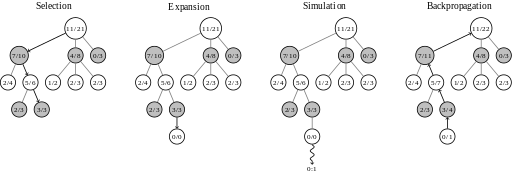
\includegraphics[width=\linewidth]{MCTS.png}
        \caption{MCTS}
        \label{fig1:Monte Carlo Tree search}
    \end{figure}
	
	Selection is the first stage in a Monte Carlo tree search. Begin with the root R and progress through the child nodes until you reach the leaf node L. The current game state is represented by the root, and a leaf is any node with a potential child but no simulation (play out) has yet been initiated. The section that follows goes into greater detail on a method of biasing the selection of child nodes that allows the game tree to expand towards the most promising moves, which is the essence of Monte Carlo tree search. Unless L finishes the game decisively (e.g., win/loss/draw) for either player, the second stage is expansion.\cite{Report} Create one (or more) offspring nodes and select node C from one of them. Any legitimate move from the game position described by L is a child node. The third stage is simulation, which is accomplished by completing one random play out from node C. This process is also known as play out or roll out. A play out could be as easy as selecting uniform random moves till the game is over (for example in chess, the game is won, lost, or drawn). Back propagation is the final stage, which uses the results of the play out to update information in the nodes on the path from C to R.
\subsection{Policy Value Network(PVN}
    A policy-value network is a type of artificial neural network that is commonly used in game-playing AI to evaluate the current state of the game and predict the best action to take. In the context of Chinese chess (Xiangqi), a policy-value network could be used as part of the static evaluation function to evaluate the current position on the board and predict the best move to make. A policy-value network typically consists of two main components: a policy network and a value network. The policy network predicts the probability of each possible action given the current state of the game, while the value network estimates the value of the current position on the board. These two components are typically trained together using a combination of supervised and reinforcement learning techniques, allowing the network to learn from a large number of game positions and outcomes. The output of the policy-value network can then be used by the game-playing AI to make more informed decisions during gameplay.
	
\section{Prior Work}
    Artificial Inteligence and Machine learning algorithm models are one of the most widely employed methods for decision and strategy projects. In this section we will focus on the prior works done in using AI and ML models implemented in other strategy games, especially the Monte Carlo tree search implementation, as it is the one of the most important part of this project 
\subsection{Alpha Go Zero}
    The game "Go" is played with a rectangular board and black and white circular pieces. There are 19 lines and 361 intersections on the regular board, and the pieces must move on the intersections where spaces are not forbidden. Because Black has a first move advantage, Black is artificially required to give White an eye at the end of the game. AlphaGo Zero is a computer software that combines a deep neural network with an advanced search tree. As an input, these neural networks process a description of the Go board through a number of network layers comprising millions of neuron-like connections. The "policy network," a neural network, chooses the next move to play. The "value network," the other neural network, predicts the game's winner. We exposed AlphaGo Zero to a variety of amateur games in order to help it build a grasp of reasonable human play. Then we let it play thousands of times against different versions of itself, each time learning from its mistakes. AlphaGo Zero evolved over time, becoming ever stronger and better at learning and decision-making. This is referred to as reinforcement learning. AlphaGo Zero went on to defeat Go world champions in many worldwide arenas, establishing himself as the greatest Go player of all time.In a Go game, AlphaGo Zero builds a local policy to sample the next move using MC Tree Search. MCTS looks for potential moves and stores the results in a search tree. As more searches are made, the tree and its information grow in size. \cite{Surag}
    
    

\subsection{Deep blue}
    Deep Blue was a chess-playing expert system that ran on a one-of-a-kind IBM supercomputer. It was the first computer to win a game and the first to win a match against a defending world champion in regular time.
    Deep Blue's evaluation function was first developed in a generalized manner, with many parameters still to be defined. Thousands of master games were analyzed to get the values for these factors. The evaluation function was then divided into 8,000 pieces, many of which were intended for specific roles. The opening book featured almost 4,000 positions and 700,000 grand master games, while the endgame database included many six-piece endgames as well as all five and fewer piece endgames. An supplementary database known as the "extended book" summarizes whole grand master games. To identify opening moves, the algorithm combines its ability to search 200 million chess positions per second with summary information from the extended book. \cite{DeepBlue}
    \begin{figure}
        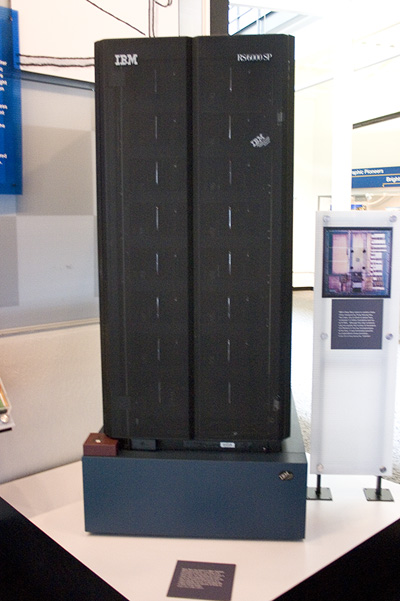
\includegraphics[width=90]{Deep_Blue.jpg}
        \caption{Deep Blue cabinets}
        \label{fig2:Deep Blue}
    \end{figure}
    
\section{Methodology}
    For this AI-Chinese chess project, I attempt using the Python programming language. The code uses the Pygame library for graphical user interface (GUI) and game board display. The game allows for a human player to play against a trained Monte Carlo Tree Search (MCTS) algorithm with a policy-value network. This goal will be done by implementing the MCTS algorithm and policy-value network with compatibility regarding the game. 
    
\subsection{Language and platform}
    In this project, I propose using Python for this project. The benefits includes simplicity and consistency, access to great libraries and frameworks for AI and Chine leaning, flexibility, and platform independence.
    
\subsection{Machine and platform}
    The entire programming and training part will be done on a windows environment-based machine. The following required versions of libraries for this program to run.
    - Python 3.x
    - Pygame 2.x
    - Tensorflow 1.x and 2.x
    - Random
    - Time
    - os 
    - Math

\subsection{Feature extractor, Policy network and Value net work}
    The who project is made up of three interconnected neural networks: a feature extractor, a policy network, and a value network. This is also why AlphaGo Zero is sometimes referred to as the two-headed beast: it has a body (the feature extractor) and two heads (policy and value). The feature extractor model generates its own board state representation. The policy model generates a probability distribution across all possible moves, while the value model generates a scalar value in the range [1;1] to signify which player is more likely to win based on the current condition of the board. The output of the feature extractor is used as input by both the policy and value models.\cite{Java}

\subsection{Monte Carlo tree search}
    \begin{itemize}
    \item Each node in the tree represents a board state and stores various statistics, including the number of times the node has been visited (n), the total action value (w), the prior probability of reaching that node (p), the mean action value (q, which is q=w/n), the move made from the parent to reach that node, a pointer to the parent node, and finally all the legal moves from this node that have a non-zero probability as children\cite{Java}.
    \item During the initial phase, the algorithm starts with a root node and chooses a child node with the highest win rate. We also want to ensure that each node has an equal probability. The goal is to keep selecting optimum child nodes until we reach the tree's leaf node. UCT is a nice approach to find such a child node\cite{Java}.
    \item Expansion: When it is unable to discover the successor node using UCT, it grows the game tree by adding all potential states from the leaf node.
    \item Following Expansion, the algorithm selects a child node at random and simulates a randomized game from the selected node until it reaches the game's resulting state. Light play out occurs when nodes are chosen at random or semi-randomly throughout the play out. You can also choose to put in a lot of effort by writing quality heuristics or evaluation functions\cite{Java}.
    \item When the algorithm approaches the end of the game, it evaluates the state to determine which player has won. It traverses upwards to the root and increases the visit score for all visited nodes. It also updates the win score for each node if the player for that position wins the play out. MCTS maintains repeating these four phases until a set number of iterations or a fixed length of time has passed. Based on random motions, we estimate the winning score for each node in this method. The greater the number of iterations, the more reliable the estimate gets. The algorithm estimations will be less accurate at the start of a search and will continue to improve after a significant length of time. Again, it is totally dependent on the nature of the problem.\cite{Dylan}
\subsection{MCTS and PVN implementation}

    First, a PVN is trained using supervised learning on a dataset of expert human moves in the Chinese Chess game. The PVN takes in a board state as input and outputs a probability distribution over the possible actions (i.e. moves) in that state. This initial PVN is used to guide the search in MCTS by providing a policy to follow.

    During MCTS, the PVN is used to evaluate the leaf nodes in the search tree. This helps to reduce the depth of the tree search and improve the efficiency of the algorithm. The PVN is also used to guide the search towards promising immediate actions, which reduces the breadth of the search from a given node.

    After the initial training of the PVN, the PVN can be fine-tuned using self-play and reinforcement learning. In this phase, the PVN plays games against itself and updates its weights using the REINFORCE algorithm. This helps the PVN to learn strategies that are optimized for winning the game, rather than just following the general pattern of action selection of expert human players.

    Finally, the trained PVN and MCTS algorithm can be used together to play the Chinese Chess game. The PVN is used to guide the search in MCTS and to evaluate the leaf nodes in the search tree. The MCTS algorithm is used to explore the tree and find the most promising actions to take in each state. This allows the PVN-MCTS combination to make more informed and optimal decisions in the game.

    In summary, MCTS is used to explore the space of possible actions in the Chinese Chess game and guide the search towards promising actions, while the PVN is used to evaluate the leaf nodes in the search tree and provide a policy for the MCTS to follow. Together, these two algorithms allow for efficient and effective decision making in the Chinese Chess game.

\subsection{Substitution plan}
    During the process of researching the background information, I have realized that, there is a possibility that the policy value network may not work out. Therefore, I have attempted to construct a static evaluation tree to do the evaluation and guidance work for the MCTS algorithm. 

    A static evaluation function is a heuristic used in game-playing AI to evaluate the game's current state and estimate its value. In the context of this Xiangqi program, the static evaluation function assigns a numerical value to the current position on the board. This value is used by the Minimax algorithm to determine the best move to make. The static evaluation function used in this program appears to simply divide the total value of all pieces on the board by a constant number 'static eval divisor' which is then used as the evaluation of the current position. This is a very basic approach to static evaluation and may not produce the most accurate or effective results in comparison to the Policy value network.

   This is my approach in the actual implementation of the static evaluation function used in the Xiangqi program. The function takes a board as input and returns the total value of all pieces on the board for each player. The value of each piece is determined using a dictionary (value dict) that assigns a numerical value to each type of piece. The function then iterates over the squares on the board and adds the value of each piece to the total material value for the corresponding player. The function also takes into account the position of the pawns (or "soldiers" in Xiangqi) by assigning them a higher value if they are on their side of the river. This implementation of the static evaluation function is a relatively simple approach that only considers the material value of the pieces on the board, and does not consider other factors such as the position of the pieces or the potential for future moves. Therefore, this approach is a substitution in case the policy value network doesn't work. 

\subsection{Evaluation}
    For the evaluation section of the PVN, my approach was simply to observe the changes that PVN shows in terms of win rate in contrast to solo the MCTS. This will be shown through a demonstration of graphs.  

    For the evaluation of the static evaluation function, since this evaluation tree will not be able to train itself, the evaluation will be done through the win rate of how many games it played with other implemented algorithms. 

\end{itemize}

\section{Over all Evaluation}
    For This project's evaluation process, I purpose that it should be evaluated in the following three methods and standards: Winning rate; Real human competition feedback; code efficiency. The goal of this evaluation process are listed in the following space:

    \begin{itemize}
    \item To evaluate the functionality of the project;
    \item To evaluate the success level of this project 
    \item To Examine possible improvements and future adjustments;
\end{itemize}
    
\subsection{Winning rate}
    This section of evaluation will be based on three separate winning rate in this project, including the winning rate of each move and each game, along with the winning rate curve through out the game. in the context of the code, this will be how stable the evaluation tree. I would like to see an constant increase of higher static value for one player. Here, we use the winning rate observed in game records instead of the "true" probability estimated by Monte Carlo Simulation by comparing it with the "true probability\cite{}. The significance of this procedure is to verify the reliability of each move's calculation. In addition to the above metrics, I would also measure the win rate of MCTS competing with other algorithms. 
    
\subsection{Real Human competition feedback}
    During this process of the evaluation, i will invite around 5-10 people and each play 10 games with the AI to test out the gaming ability of the AI. In addition, i will ask players to provide a feedback survey based on the experience, difficulty, and improvements of the AI. This is essential, because the program is design to assist people to train themselves. Thus, user experience is extremely important. 
    
\subsection{Comparison of Performance in other implementation of Monte Carlo implementation}
    In this last process of evaluation, i propose to compare the performance outcome based on accuracy, precision, F-score, win rate and performance time with Alpha Go, and other Monte Carlo implementations on chess and Shigo. The meaning of this process is to evaluate whether  this project successes in matching other projects performance or not. As well as to find weak spots to improve\cite{Accuracy}
    In the context of this project, i will compete the MCTS with, a MCT algorithm driven by a q value search tree, a random search tree, and another MCTS player. 
    

\section{Results and Discussion}
    This section documents the results in attempting to create a self-learnable AI in the context of a Chinese chess game that utilizes the MTCS algorithm and policy value network which is designed to predict the best move. The result and relevant discussion will be shown in the following subsections. 
\subsection{Functionality}
    I was able to provide a fully functional Chinese chess game write in python 3. The program successfully implemented the following functions 
        \begin{itemize}
    \item Able to allow a user to assign two players with the following option; human.player, mcts.player, random.player, All these three options are able to be assigned to both red and black player. This can be modified in the init() function in CCMCTS.py file.;
    \item Able to generate a move through a static evaluation of the current board state.;
    \item Able to allow the MCST to use the static evaluation divisor and calculated UCB value to determine the next best move;
    \item Able to generate the current game state, moves made, and legal move suggestions for the current player. It also can save the printed game progress and result in a separate directory. ;
    \item the program has a complete functional GUI and visual representation of the Chinese chess game board where the user can play the game by user their mouse. The current game state will be printed in the command prompt along with the progression of the game. ;
    \item The program did include a policy value network code in it. However, due to the limitation and restrictions, i was unable to install TensorFlow on either one of my machine. Therefore i wasn't able to train the policy value network. After spending way to long on trying to get tensorflow work on my machine, i choose to continue my project with the back-up plan by using a static evaluation tree function instead. This issue directly resulted in that i failed in creating an self-learning AI-Chinese chess engine. However with the implementation of live static evaluation function, the program can still use the static eval divisor based on current game state and the evaluation on every iterations of the mcts algorithm loop to provide both aggressive and defensive moves with the best outcomes. ;
    \item The program and the mcts fully follow and adapted to the Chinese chess rule provided by Wikipedia which i find most online Chinese chess engine uses. ;
    \item I have also included an older version of the chinese chess game that i create using a Q-value search tree based on a MCT algorithm introduced by the Alpha Go team. I had to abaddon this version due the the fact that i hard-coded the game's chess logic and rules in the human player and mct player. This limits the program to selfplay in bot vs bot mode. However i did use this engine to play against the update version. It ended up that the Updated version of the game show a significant higher win rate. ;
\end{itemize}
    After examine how machine-played Xiangqi differs from human-played Xiangqi using the Monte Carlo tree search (MCTS) algorithm and implementing a separate policy value network in the Chinese chess game to increase the chess' ability to provide the best moves. The MCTS algorithm is used to simulate chess moves and select the best winning rate strategy, while the static evaluation function assigns a value to a specific position in the game. This value represents the estimated strength of a player's position based on various factors, such as the number and type of pieces, the control of key squares or positions on the board, and the pawn structure. The static evaluation function is used to evaluate positions at a particular point in the game, without considering future moves or potential variations. It is typically used in conjunction with search algorithms, such as minimax or alpha-beta pruning, to help the AI player determine the best move to make in a given position. The static evaluation function can be implemented in a number of ways, depending on the specific game and the desired factors to consider in the evaluation. using self-play and reinforcement learning to improve the chess' ability to provide the best moves. The final model combines the outputs of the MCTS algorithm and the policy value network to output the probability of each move and the winning rate of the player who makes the first move. This model can then be used to play Xiangqi against human players or other AI models.

    he Monte Carlo tree search (MCTS) algorithm is a search algorithm used to find the optimal moves in decision-making problems, such as chess and other strategy games. It works by simulating multiple potential moves and evaluating the resulting positions using a static evaluation function or some other method of estimation. The algorithm then uses the resulting evaluations to guide its search and ultimately choose the best move.

    Here is a step-by-step breakdown of the MCTS algorithm:

    Select: Starting from the root node of the search tree, the algorithm selects successive child nodes until it reaches a leaf node (a node without any children). This is done by traversing the tree using a selection policy, which determines which child node to explore next based on various factors such as the number of visits, the evaluation of the nodes, and the balance between exploration and exploitation.
    Expand: Once a leaf node is reached, the algorithm expands the node by adding one or more child nodes representing the possible moves that can be made from that position.
    Simulate: For each newly expanded child node, the algorithm simulates the remainder of the game by randomly choosing moves until the game ends. The result of the simulation (win, loss, or draw) is used to update the node's evaluation.
    Backpropagate: The algorithm then backpropagates the results of the simulation from the leaf node back up to the root node, updating the evaluations of the nodes along the way.
    Repeat: The algorithm repeats these steps for a certain number of iterations or until a time limit is reached. After the search is complete, the algorithm chooses the child node of the root node with the highest evaluation as the optimal move.
    It is important to note that the MCTS algorithm is probabilistic in nature and does not guarantee that the optimal move will always be found. However, it has proven to be very effective in many decision-making problems and is widely used in AI research and development.

    I have also tried to implement the PVN class in the code attached. It is a convolutional neural network designed to output both a policy and a value given an input tensor. The policy represents the probability distribution over all possible moves at each position on the board, while the value represents the predicted outcome of the game (win or loss).

    
\subsection{Efficiency}
    The current efficiency of MCTS is at an average responding time at 25-30 seconds. This results from setting the iteration of MCTS at 10 times with 5 layers of depth in the static evaluations tree with 1200 playouts. 
    In contrast to the average 120-second response time during the first version of my code. I have tried to improve the efficientcy by modefiying the code so that it can utilize the resouce of my GPU to do the calculation. However, do to the reason that i couldn't get CUDA tool kit access from NIVIDA due to budget reasons. I was not able to get an efficiency boost from my GPU. 
    
\subsection{Evaluation}
    Overall, the result program provide a fully functional chinese chess game that did not met the primary goal of creating a self-learning and self-improve AI model of chinese chess game. However, i did provide a substitution plan that uses a static evaluation function to replace the policy value network. The user is able to play against the AI bot players preset. 
    After examining how the MCTS moves are generated, from a human player perspective, i can see that the algorithm plays purely based on the evaluated probabilities calculated by machine and the current board evaluation. Whereas humans would use different strategies to either attack or defense. For instanse, the cannon piece in the game is a very important attacking piece. A human player usually protects it until the moment the player needs to abbandon the peice. The MCTS algorith occasionally shows that it will abbandon the piece ealy in the game trying to an early advantage in the static evaluatation tree to result in a better game state than the previous move. This is a significant sign of how Algorithm plays completely different than human players' chess game decision making logic. 

    I have tested the mcts algorithm by running it against with another MCTS player for 200games, against a random tree player for 200 games, and against a Q-value search tree for 200 games, the results are listed below:
    \begin{itemize}
        \item Against MCTS win:92 loss:75 draw:33
        \item Against Random win:196 loss:1 draw:3
        \item Against Q-Value win:162 loss:21 draw:17
    \end{itemize}
    IN summary of the result, the win rate of designed MCTS algorithm for this Chinese chess is pretty high in this relatively simple algorithm competition. It does prove the statement of MCTS is so far one of the best algorithms to use to solve decision making games. 
    
\subsection{Human player feedback}
    I invited 5 anonymous players to each play 10 games with the MCTS algorithm using my machine. The are 3 beginner players and 2 intermediate players. the result are listed below 
    \begin{itemize}
        \item P1(beginner): win:4 lose:5 draw:1
        \item P2(beginner): win:6 lose:4 draw:0
        \item P3(beginner): win:2 lose:7 draw:1
        \item P4(intermediate): win:7 lose:3 draw:0
        \item P5(intermediate): win:2 lose:5 draw:3
    \end{itemize}
    As the result shows, with the increase of the human players' elo level, it becomes harder for the mcts to win a game. However, the program does obtain the capacity in winning the majority of the games in playing against beginner players. In addition to the result this user testing session, i received an sugesstion on provide a repetition moves checker in the program. Player num5 discovered that the game moves generated by the mcts algorithm often leads to an un resolvable ending where the two opossition can continue repeating the same move without possible check mate moves. So based on user feedback, i was able to add a repetition moves detector and use it to call a draw when there are no possible end game solution or possible legal moves. 

    
    
\subsection{Ethical Evaluation}
There are a number of ethical considerations to consider when designing and implementing a chess game AI engine. Some of the key considerations include:

Fairness and impartiality: It is important to ensure that the AI engine does not have any biases or preferences that could influence its decisions and actions during gameplay. This could involve designing the AI to make decisions based solely on the current state of the game and the rules of chess, without any preconceived notions or preferences.

Transparency and explainability: It is important for the AI engine to be transparent and explainable, so that players and other stakeholders can understand how it makes decisions and why it makes certain moves. This could involve providing explanations for each move the AI makes, or allowing players to access the AI's internal decision-making process to gain a better understanding of its behavior.

Impact on human players: The AI engine should be designed to have a positive impact on human players, rather than undermining their ability to play the game or making the game less enjoyable for them. This could involve designing the AI to provide a challenging but fair opponent for human players, or providing tools and resources that can help human players improve their skills and strategies.

Privacy and security: It is important to ensure that the AI engine does not compromise the privacy or security of players or other stakeholders. This could involve implementing appropriate security measures to protect players' data and personal information, and ensuring that the AI engine does not access or use any sensitive information without permission

    
\section{Ethical Consideration}
    The world is almost driven by technologies today, countless innovative products are being invented and introduced to people every day. When the project is designed with ethical and moral standards, it is essential to prevent unequal, unethical, injustice, and harmful events from happening. During the early stages of computer technology, ethical concerns about computers were virtually non-proposet because computers were not nearly as complex as they are now. However, ethical circums,ances about computers and cyber ,echnology aproposeoidable in contemporary civilization. Computer technology permeates every area of our daily life. Different computer technology offers distinct capabilities implementationsople to carry out daily tasks effectively and quickly. In recent decades, computer scientists have been trying to produce multiple machine learning AI in chess games and other competitive sports in favor of testing the limitations of both humanthroughoutnes. We now live in a world dominated by capitalism and advanced technology. With the more advanced science and technologies, humans tend to apply these techs in various fields to save cost or provide convenience. However, while technologies such as AI is being implemented in different areas, different ethical consideration must be considered and create precautions for it. This paper will examine ethical issues, including power, accessibility, resource consumption, upkeep, and maintenance.
\subsection{General Ethical consideration}
    The general ethical discussion going on for years is should AI exist? Scientists and the general public hais designedsed this controversial topic for decades. Simple AI and machine learning can provide people convenience in daily life, such as making a living easier using AI-controlled intelligent home devices. More complicated AI may be applied to auto-driving cars or search engines to provide more accurate search results. Scientists even pushed the limitation of AI into making decisions for humans. For instance, A corporate institution may use AI to help them select the employees they need. A college may use AI to filter out those students who aren't qualified for their standards. A court may use AI to judge human crimes based on laws. These examples demonstrate that with the advancement of AI technology to this day, it can replace humans in many positions while providing more efficiency to work. Machines, robots, and algorithms are slowly replacing some people's positions in modern society. The creators and users of AI must set ethical and moral standards for these technologies if the AI trend is unstoppable\cite{EthicalIssue}. It is clear that ethics are not only vital but also critical in reshaping these powerful algorithms in favor of humanity. Machines learn ethics through the programming that is programmed into them. As a result, the creators of these so-called AI algorithms should not take this lightly. Where we are today is the result of millions of years of evolution. When compared to the development of AI fields, we are not nearly a century old since the first computer was invented. The internet is only three decades old. So you can picture the rate of change in the world of artificial intelligence. Without ethics, a field as fast-paced as this would spell tragedy if it fell into the wrong hands\cite{BillGates}.
    
\subsection{Power Consideration}
    There is a potential power ethic issue in the project of training an AI to learn and mimic the human mindset in playing chess. The power issue strands for providing some or a group of people unequal power over others. As a project part of the trend of AI and machine learning, this project potentially acts as a small part of the grand scheme. While the ability of AI can beat the best of humans in other board games, such as Alpha GO winning Lee Sedol in the 'GO' game during the 2016 march, it inspired others to do the same in other chess or board games\cite{AlphaGo}. Even real sports as everyone knows that chess board games and any other sports games are supposed to be fair to play. In the context of this paper, the Chinese chess game should be assumed to be honest and unbiased. With the pandemic happening, more and more people choose to play the Chinese chess game online and compete with other players. A small group of people uses AI to help them win higher-rank games, resulting in a series of unfair games. Evidently, YouTube held dozens of video tutorials on using Online AI to cheat in online chess games. This potentially distributes power to those who use AI in online competitions, Which could be defined as cheating. Moreover, the player playing against those cheaters may have no idea about that, resulting in a bad mood and even doubting their abilities in playing the game. The charming part of a competitive game is about both winning and losing. If someone is only there to experience loss, it may cause them to quit the game forever. This type of cheating is unethical and unacceptable and wholly abandoned the common sense of maintaining a fair competition game environment. The purpose of creating this AI Chinese chess project is to help train players' chess skills while practicing it. Using this project to cheat in online competition games should not be tolerated, yet there are only a few ways to prevent this from happening. The solution found is limited but could potentially be helpful. 

\subsection{Environmental consideration}
    While AI is learning how the human brain functions and uses it to either assist people in work, life, or provide entertainment, these AI's consume tons of energy resources to train the model and cause environmental concerns. For instance, on 45 terabytes of data, OpenAI trained its GPT-3 model. According to the US Energy Information Administration, the average household uses 10,649 kWh per year. As a result, training the final version of MegatronLM consumed nearly the same amount of energy as three homes use in a year\cite{EnergyConsumption}. The heavier the data set is used to train, the more energy and resources it consumes. As the trend of AI rises, a great deal of AI models has been developed and trained in recent decades. Even though these AI models may contribute to society, individuals, or organizations in certain ways, the creator must not ignore the potential environmental issues it creates. The increased use of resources may cause a more toxic environment on Earth and speed up climate change. Consume energy results in the production of CO2, the principal greenhouse gas released by humans. In the atmosphere, greenhouse gases such as CO2 trap heat at the Earth's surface, increasing the Earth's temperature and upsetting sensitive ecosystems. Protecting the environment should be everyone's responsibility. Under the condition that training artificial intelligence models contributes to the advancement of human society and technology, scientists must consider optimizing algorithms and data usage to reduce the training capacity and energy consumption. The AI-Chinese chess project tries to use the minimum data required to train the model and use renewable energy to reduce CO2 emissions. Just as McGovern said, "we must factor in the earth experience" while creating and training AI.  

\section{Future improvements}
    After implementing an artificial intelligence (AI) system for playing the board game Xiangqi (also known as Chinese chess) using a combination of Monte Carlo Tree Search (MCTS) and attempt to implement a policy value network. in the future i wish i could modify the code so that the AI system uses MCTS to explore the space of possible moves and estimates the value of each move based on the outcomes of simulated playouts. It also uses a deep convolutional neural network (CNN) to predict the likelihood of each move and the current player's victory rate, and a policy value network to predict the probability of winning given the current game state and the expected value of each move.

    The authors evaluated the performance of the AI system using various metrics, including win rate against a strong commercial Xiangqi AI program and win rate against human players. They found that the AI system performed well, but there is still room for improvement.

    One potential direction for future work could be to explore ways to further improve the performance of the AI system, such as by fine-tuning the CNN and policy value network architectures, using more advanced training techniques, or incorporating additional sources of information into the AI system. Another possibility could be to investigate the use of alternative algorithms or techniques, such as reinforcement learning or evolutionary computation, to further improve the ability of the AI system to learn and adapt to new situations. Finally, it could be interesting to explore how the AI system performs in different types of Xiangqi games, such as faster-paced games or games with different starting positions, to see if there are any specific areas where the AI system could be further improved.





\printbibliography 


\end{document}